\documentclass[aspectratio=169, 12pt]{beamer}

\usetheme[progressbar=frametitle]{metropolis}
\usepackage{appendixnumberbeamer}

\usepackage{booktabs}
\usepackage{adjustbox}
\usepackage{svg}
\usepackage{tikz}
\usepackage{hyperref}
\usepackage[scale=2]{ccicons}
\newcommand{\ra}[1]{\renewcommand{\arraystretch}{#1}}

\usepackage{pgfplots}
\usepgfplotslibrary{dateplot}

\usepackage{xspace}
\newcommand{\themename}{\textbf{\textsc{metropolis}}\xspace}

\title{Forex Forecasting}
\subtitle{Combining statistical methods with neural networks}
% Authors
\author{Efstathios Kotsis \inst{1} \and Michael Darmanis \inst{1} \and Vasilios Venieris \inst{1}}
% Affiliations
\institute{\inst{1} National and Kapodistrian University of Athens}
% Date
\date{\today}
% \institute{Center for modern beamer themes}
% \titlegraphic{\hfill\includegraphics[height=1.5cm]{logo.pdf}}

\begin{document}

\maketitle

\begin{frame}{Time Series \& Time Series Forecasting}
    \begin{columns}[T] % align columns
        \begin{column}{.5\textwidth}
            \begin{itemize}
                \item \textbf{Time series} are observations taken sequentially in time.
                \item \textbf{Time series forecasting} predicts future values based on past (historical data).
            \end{itemize}
        \end{column}
        
        \begin{column}{.5\textwidth}
            \begin{tabular}{|l|r|}
                \hline
                Date & Observation \\
                \hline
                2018-06-09 & 64 \\
                2018-06-10 & 66 \\
                2018-06-11 & 69 \\
                2018-06-12 & 72 \\
                \hline
                2018-06-13 & ? \\
                2018-06-14 & ? \\
                \hline
            \end{tabular}
            
        \end{column}
    \end{columns}
\end{frame}


\begin{frame}{Why Deep Learning Models?}
    \begin{itemize}
    \item Deep learning models have shown to perform well in many forecasting scenarios
        \begin{itemize}
            \item 2014 Global Energy Forecasting Competition (\href{https://www.crowdanalytix.com/contests/global-energy-forecasting-competition-2014-probabilistic-electricity-price-forecasting}{link})
            \item 2016 CIF International Time Series Competition (\href{https://irafm.osu.cz/cif/main.php}{link})
            \item 2017 Web Traffic Time Series Forecasting (\href{https://www.kaggle.com/c/web-traffic-time-series-forecasting#timeline}{link})
            \item 2018 Corporacion Favorita Grocery Sales Forecasting (\href{https://www.kaggle.com/c/favorita-grocery-sales-forecasting}{link})
            \item 2018 M4-Competition (\href{https://forecasters.org/blog/2017/12/21/m4-competition-1-1-2018/}{link})
        \end{itemize}
    
    \item Non-parametric
    \item Flexible and expressive
    \item Easily inject exogenous features into the model
    \item Learn from large time series datasets
\end{itemize}

\end{frame}

\begin{frame}{Scenario: Forex Forecasting}
    \begin{itemize}
        \item Forex is the global marketplace for trading national currencies against one another, operating 24/5.
        \item  Here, we'll use the European's Central Bank (ECB) dataset for various currencies against the euro
    \end{itemize}
\begin{table}[h]
\centering
\caption{ECB forex dataset}\label{tab:data}
\begin{tabular}{ccccccc}
\toprule
\textbf{Date} & \textbf{USD} & \textbf{JPY} & \textbf{BGN} & \textbf{...} & \textbf{THB} & \textbf{ZAR} \\
\midrule
2023-09-15 & 1.0658 & 157.50 & 1.9558 & ... & 38.145 & 20.2968 \\
2023-09-14 & 1.0730 & 158.13 & 1.9558 & ... & 38.387 & 20.3109 \\
... & ... & ... & ... & ... & ... & ... \\
1999-01-04 & 1.1789 & 133.73 & NaN & ... & NaN & 6.9358 \\
\bottomrule
\end{tabular}
\end{table}
\end{frame}

\begin{frame}{Dataset considerations}
    \begin{itemize}
        \item \textbf{Missing Values:} Require careful imputation to avoid bias.
        
        \item \textbf{Data Frequency:} Daily data, resampling needed for other frequencies.
        
        \item \textbf{Currency Pairs:} Challenge in selecting relevant pairs.
        
        \item \textbf{Normalisation:} Essential for data comparability.
        
        \item \textbf{Non-Trading Days:} Adjustments necessary for continuity.
        
        \item \textbf{Time Zones:} ECB's CET time zone updates impact intra-day rates.
        
        \item \textbf{Institutional Bias:} ECB interventions can cause rate discrepancies.
    \end{itemize}

All series were adjusted to a fixed length, ensuring consistency for effective vectorisation.
\end{frame}

\begin{frame}[allowframebreaks]{Approach and Assessment}

\begin{itemize}
        \item Used forecasting methods to supplement a Convolutional Neural Network (S-CNN).
        \begin{itemize}
            \item \textbf{Why?} To Address the non-linear nature of Forex data.
        \end{itemize}
        \item Adopted a traditional forecasting method as the foundation, and enhanced it with a Recurrent Neural Network (ES-RNN).
        \begin{itemize}
            \item \textbf{Why?} To Addressed the linear trend assumption of the forecasting method\cite{ayitey}.
        \end{itemize}

\begin{center}
    \textsc{\textbf{Benchmarking}}
\end{center}
        
Used a VAR (Vector Autoregressive) model for performance comparison and benchmarking.
\end{itemize}

sMAPE (symmetric Mean Absolute Percentage Error) was used to assess the models

\[
\text{sMAPE} = \frac{200\%}{n} \sum_{t=1}^n \frac{|F_t - A_t|}{|F_t| + |A_t|},
\]

where 
\begin{itemize}
    \item $F_t$ is the forecasted value at time $t$,
    \item $A_t$ is the actual value at time $t$,
    \item $n$ is the total number of observations.
\end{itemize}

\end{frame}

\section{Smoothed Convolutional Neural Network (S-CNN)}

\begin{frame}{S-CNN: Origin and basic idea}
    \begin{itemize}
        \item Implementation based on the paper ``Time-series analysis with smoothed Convolutional Neural Network''\cite{e-cnn} (no available code) .
        \item Model is univariate, multi-step.
        \item Simple exponential smoothing (remove outliers, average) + CNN.
    \end{itemize}
\end{frame}

\begin{frame}[allowframebreaks]{S-CNN: Simple Exponential Smoothing}
  \begin{equation*}
    \displaystyle s_{t}=\alpha x_{t}+(1-\alpha )s_{t-1}=s_{t-1}+\alpha (x_{t}-s_{t-1})
  \end{equation*}
    \begin{itemize}
        \item For $\alpha$ values close to 1 we get very little influence of the previous smoothed value.
        \item For $\alpha$ close to 1 we also see that the previous unsmoothed series observation influences the result more than the smoothed values.
        \item For the calculation of $\alpha$, since there is no golden rule, we adopted the $\alpha$ value from the aforementioned publication.
        \item In particular the authors argue that $\alpha$ should be dependent on the dataset and must be of course between 0 and 1. Also the average value of the series should be less than the difference between max and min.
    \end{itemize}
So we end up with the following formula
\begin{equation*}
\alpha_{\text{opt}} = \frac{\left( X_{\text{max}} - X_{\text{min}} \right) - \frac{1}{n} \sum_{t=1}^{n} X_t}{X_{\text{max}} - X_{\text{min}}},
\end{equation*}
and the simple smoothing becomes
\begin{equation*}
s_t = s_{t-1} + \frac{\left( x_{\text{max}} - x_{\text{min}} \right) - \frac{1}{n} \sum_{t=1}^{n} x_t}{x_{\text{max}} - x_{\text{min}}} \left( x_t - s_{t-1} \right) .
\end{equation*}
\end{frame}

\begin{frame}{S-CNN: Architecture}
Basic architecture from Wibawa et al.\cite{e-cnn} and experimented with different number of hidden layers.
\begin{figure}[htbp]
\centering
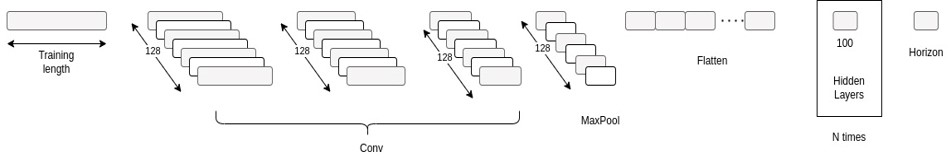
\includegraphics[width=\columnwidth]{./plots/s-cnn.jpg}
\end{figure}
\begin{center}
    Kernel size: $1x2$, Stride: $1x1$
\end{center}
\end{frame}

\begin{frame}[allowframebreaks]{S-CNN: Training}
    \begin{center}
    \textsc{\textbf{How to pick the number of hidden layers?}}
    \end{center}
    We used the Lucas numbers suggested. They derive from the Fibonacci Sequence if instead of adding every 2 successive observations we skip the intermediate and add the K with the K+2 together.
    \begin{figure}[htbp]
    \centering
    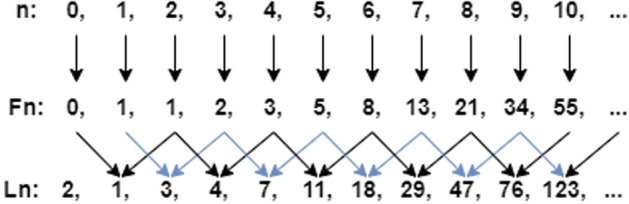
\includegraphics[width=0.6\columnwidth]{./plots/fibonacci.jpg}
    \end{figure}

Model yielded the lower MSE, for the most stable currencies, for 76 layers of training.

\begin{table}[htbp]
\centering
\caption{Training time for different numbers of hidden layers}
\begin{tabular}{cc}
\toprule
Number of Hidden Layers & Training Time (hh:mm:ss) \\
\midrule
3 & 0:27:43.15 \\
11 & 0:34:27.77 \\
47 & 1:05:21.78 \\
76 & 1:28:47.70 \\
\bottomrule
\end{tabular}
\end{table}
\begin{center}
    \textsc{\textbf{Training steps...}}
\end{center}
\begin{itemize}
\item Split the dataset into series of different frequencies.
\item For each time series we normalise + smooth.
\item Feed the output into the convolutional model and train the model to predict a horizon of K steps for this frequency, where K is a model’s designers choice.
\end{itemize}
\newpage
\begin{center}
    \textsc{\textbf{Training history.}}
\end{center}
In order to balance training with only recent data, or feeding with irrelevant outdated history, we train with a list of possible training lengths.
\begin{itemize}
    \item Daily: [14, 20, 240]
    \item Weekly: [52, 13, 26]
    \item Monthly: [24, 18]
    \item Quarterly: [12, 8]
    \item Yearly: [6]
\end{itemize}
\newpage
\begin{center}
    \textsc{\textbf{Train/validation/test split.}}
\end{center}
\begin{itemize}
    \item We focused on data after 2010 since in 2008 – 2010 there was the European debt crisis. A plot from the data can show that the economy and the currency fell rapidly in most countries in the European continent and in many other countries.
    \item For the frequencies except Yearly, we trained with splits of 80\%-20\%, 70\%-30\%, and approximately 60\%-40\% for quarterly (training/validation).
    \item We split the dataset accordingly and fed the created datasets to the generators.
    \item The models were trained for 200 epochs, using the MSE loss function and the Adam optimiser.
\end{itemize}

\end{frame}

\begin{frame}[allowframebreaks]{S-CNN: Results}
For stable currencies, longer training tends to yield more accurate predictions.
\begin{table}[htbp]
\centering
\caption{sMAPE for Daily with 76 Hidden Layers (Biggest Lucas Number Tested)}
\begin{tabular}{lcc}
\toprule
& \multicolumn{2}{c}{SMAPE} \\
\cmidrule{2-3}
& Training length 20 days & Training length 240 days \\
\midrule
CAD & 104.24 & 26.63 \\
AUD & 226.39 & 79.63 \\
DKK & 1.357 & 0.937 \\
\bottomrule
\end{tabular}
\end{table}
Unpredictable currencies benefit from short-term history and possibly higher $\alpha$ for forecasting. More hidden layers may overfit. Fewer hidden layers excel for daily predictions of unstable currencies.
\begin{table}[htbp]
\centering
\caption{sMAPE for 76 Hidden Layers}
\begin{tabular}{lcccc}
\toprule
& \multicolumn{4}{c}{sMAPE} \\
\cmidrule{2-5}
& T.L. 20 days & T.L. 240 days & T.L. 8 quarters & T.L. 12 quarters \\
\midrule
USD & 59.67 & 138.76 & 72.69 & 82.30 \\
\bottomrule
\end{tabular}
\end{table}
Quarterly and monthly predictions outperform daily ones for stable currencies. Daily and weekly forecasts show many fluctuations and are less accurate.
\begin{columns}
    \begin{column}{0.25\textwidth}
        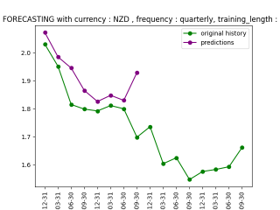
\includegraphics[width=\linewidth]{plots/r1.png}
    \end{column}
    \begin{column}{0.25\textwidth}
        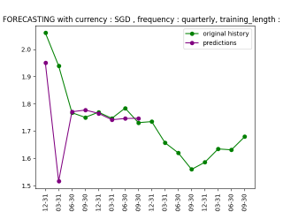
\includegraphics[width=\linewidth]{plots/r2.png}
    \end{column}
    \begin{column}{0.25\textwidth}
        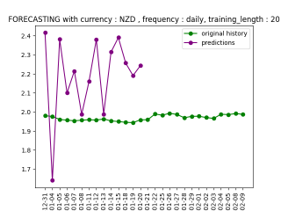
\includegraphics[width=\linewidth]{plots/r3.png}
    \end{column}
    \begin{column}{0.25\textwidth}
        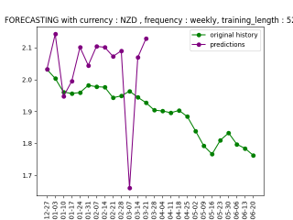
\includegraphics[width=\linewidth]{plots/r4.png}
    \end{column}
\end{columns}
\newpage

Model struggles with unpredictable currencies like \textit{USD} and \textit{GBP}.
\begin{columns}
    \begin{column}{0.5\textwidth}
        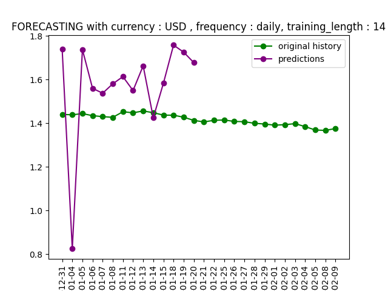
\includegraphics[width=\linewidth]{plots/usd-d.png}
    \end{column}
    \begin{column}{0.5\textwidth}
        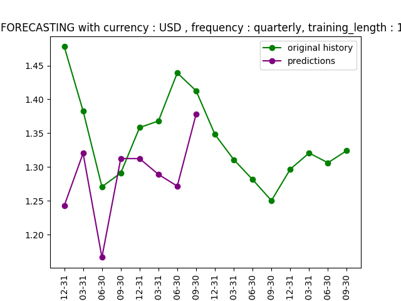
\includegraphics[width=\linewidth]{plots/usd-r.png}
    \end{column}
\end{columns}

\end{frame}

\section{Exponentially Smoothed Recurrent Neural Network}

\begin{frame}{ES-RNN: Origin and basic idea}
\begin{itemize}
    \item Implementation based on Slawek Smyl\cite{slawek}, 2018
\url{https://eng.uber.com/m4-forecasting-competition/}, Winner of M4 competition\cite{m4} (code available in C++)
    \item Use the Holt-Winters equations\cite{winters}, and replace the trend with an RNN.
\end{itemize}
\end{frame}

\begin{frame}{ES-RNN: Holt-Winters model}
Break down the problem of forecasting into three distinct equations:
\begin{itemize}
    \item level, $l_t (\alpha)$
    \item trend, $b_t (\beta)$
    \item seasonality, $s_{t} (\gamma)$ 
\end{itemize}
Optimisation problem with respect to $\alpha, \beta, \gamma$.
\begin{center}
    \textsc{\textbf{Issue: Formulation works for a linear trend.}}
\end{center}
So plug in RNN for the trend component $b_t (\beta)$.
\end{frame}

\begin{frame}{ES-RNN: Holt-Winters model (multiplicative)}
\begin{align}
    l_t &= \alpha(\frac{y_t}{s_{t-m}}) + (1 - \alpha)l_{t-1} b_{t-1} \label{eq:level}\\
    b_t &= \beta(\frac{l_t}{l_{t-1}}) + (1- \beta) b_{t-1} \label{eq:trend} \\ 
    s_{t} &= \gamma \frac{y_t}{l_{t-1} b_{t-1}} + (1-\gamma)s_{t-m} \label{eq:season}\\
    \Hat{y}_{t+h} &= l_t  b_t^h s_{t-m+h^+_m} \label{eq:predEq}
\end{align}

Equation \ref{eq:trend} is replaced by an RNN from the model as follows:
\begin{align}
    \Hat{y}_{t+1 \dots t+h} &= RNN(X_t) * l_t * s_{t+1 \dots t+h} \label{eq:modifiedEq}\\
    x_i &= \frac{y_i}{l_t s_i} \label{eq:x}
\end{align}
\end{frame}

\begin{frame}{ES-RNN: Holt-Winters model (additive)}
\begin{align}
    l_t &= \alpha (y_t - s_{t-m}) + (1 - \alpha) (l_{t-1} + b_{t-1}) \label{eq:level1}\\
    b_t &= \beta (l_t - l_{t-1}) + (1- \beta) b_{t-1} \label{eq:trend1}\\ 
    s_t &= \gamma (y_t - l_{t-1} - b_{t-1}) + (1-\gamma) s_{t-m} \label{eq:season1}\\
    \hat{y}_{t+h} &= l_t + h \cdot b_t + s_{t-m+h (\bmod m)} \label{eq:predEq1}
\end{align}

Equation \ref{eq:trend1} is replaced by an RNN in the model as follows:
\begin{align}
    \hat{y}_{t+1 \dots t+h} &= RNN(X_t) + l_t + s_{t+1 \dots t+h} \label{eq:modifiedEq1}\\
    x_i &= y_i - l_t - s_i \label{eq:x1}
\end{align}

\end{frame}

\begin{frame}[fragile]{ES-RNN: Architecture}
    \begin{figure}[htbp]
    \centering
    \def\svgwidth{\columnwidth}
    \includesvg{./plots/es-rnn.svg}
    \end{figure}
\end{frame}

\begin{frame}{ES-RNN: Training}
Used a sliding window. Input and output windows were of constant size. Output size matched the prediction horizon, while input size determined heuristically.
\begin{center}
    \textsc{\textbf{Loss Function?}}
\end{center}
Considered the L1 difference as similar enough to sMAPE; both are mean absolute differences between forecasted and actual values.
\begin{center}
    \textsc{\textbf{Experimented with}}
\end{center}
    \begin{itemize}
        \item Both multiplicative and additive Holt-Winters formulations.
        \item A simple GRU with various hidden state features (8, 16, 32), i.e. input-window size.
    \end{itemize}
\end{frame}

\begin{frame}[allowframebreaks]{ES-RNN: Results}
Multiplicative Holt-Winters is better suited; best results were achieved using an input window of 8.
\begin{table}\centering
\ra{1.3}
\caption{Averaged sMAPE(\%) values for daily and Weekly Frequencies}
\begin{adjustbox}{width=0.35\textwidth}
\begin{tabular}{@{}rrcr@{}}\toprule
& Daily && Weekly\\
\midrule
\textit{Additive Holt-Winters} \\
Input=8 & 23.45 && 17.89\\
Input=16 & 36.72 && 21.63\\
Input=32 & 28.83 && 19.42\\
\textit{Multiplicative Holt-Winters} \\
Input=8 & 13.72 && 7.96\\
Input=16 & 18.25 && 11.37\\
Input=32 & 16.92 && 9.84\\
\bottomrule
\end{tabular}
\end{adjustbox}
\end{table}
\newpage
    \begin{center}
        \textbf{L1 as the training loss function created a positive bias.}
    \end{center}
\begin{columns}
    \begin{column}{0.25\textwidth}
        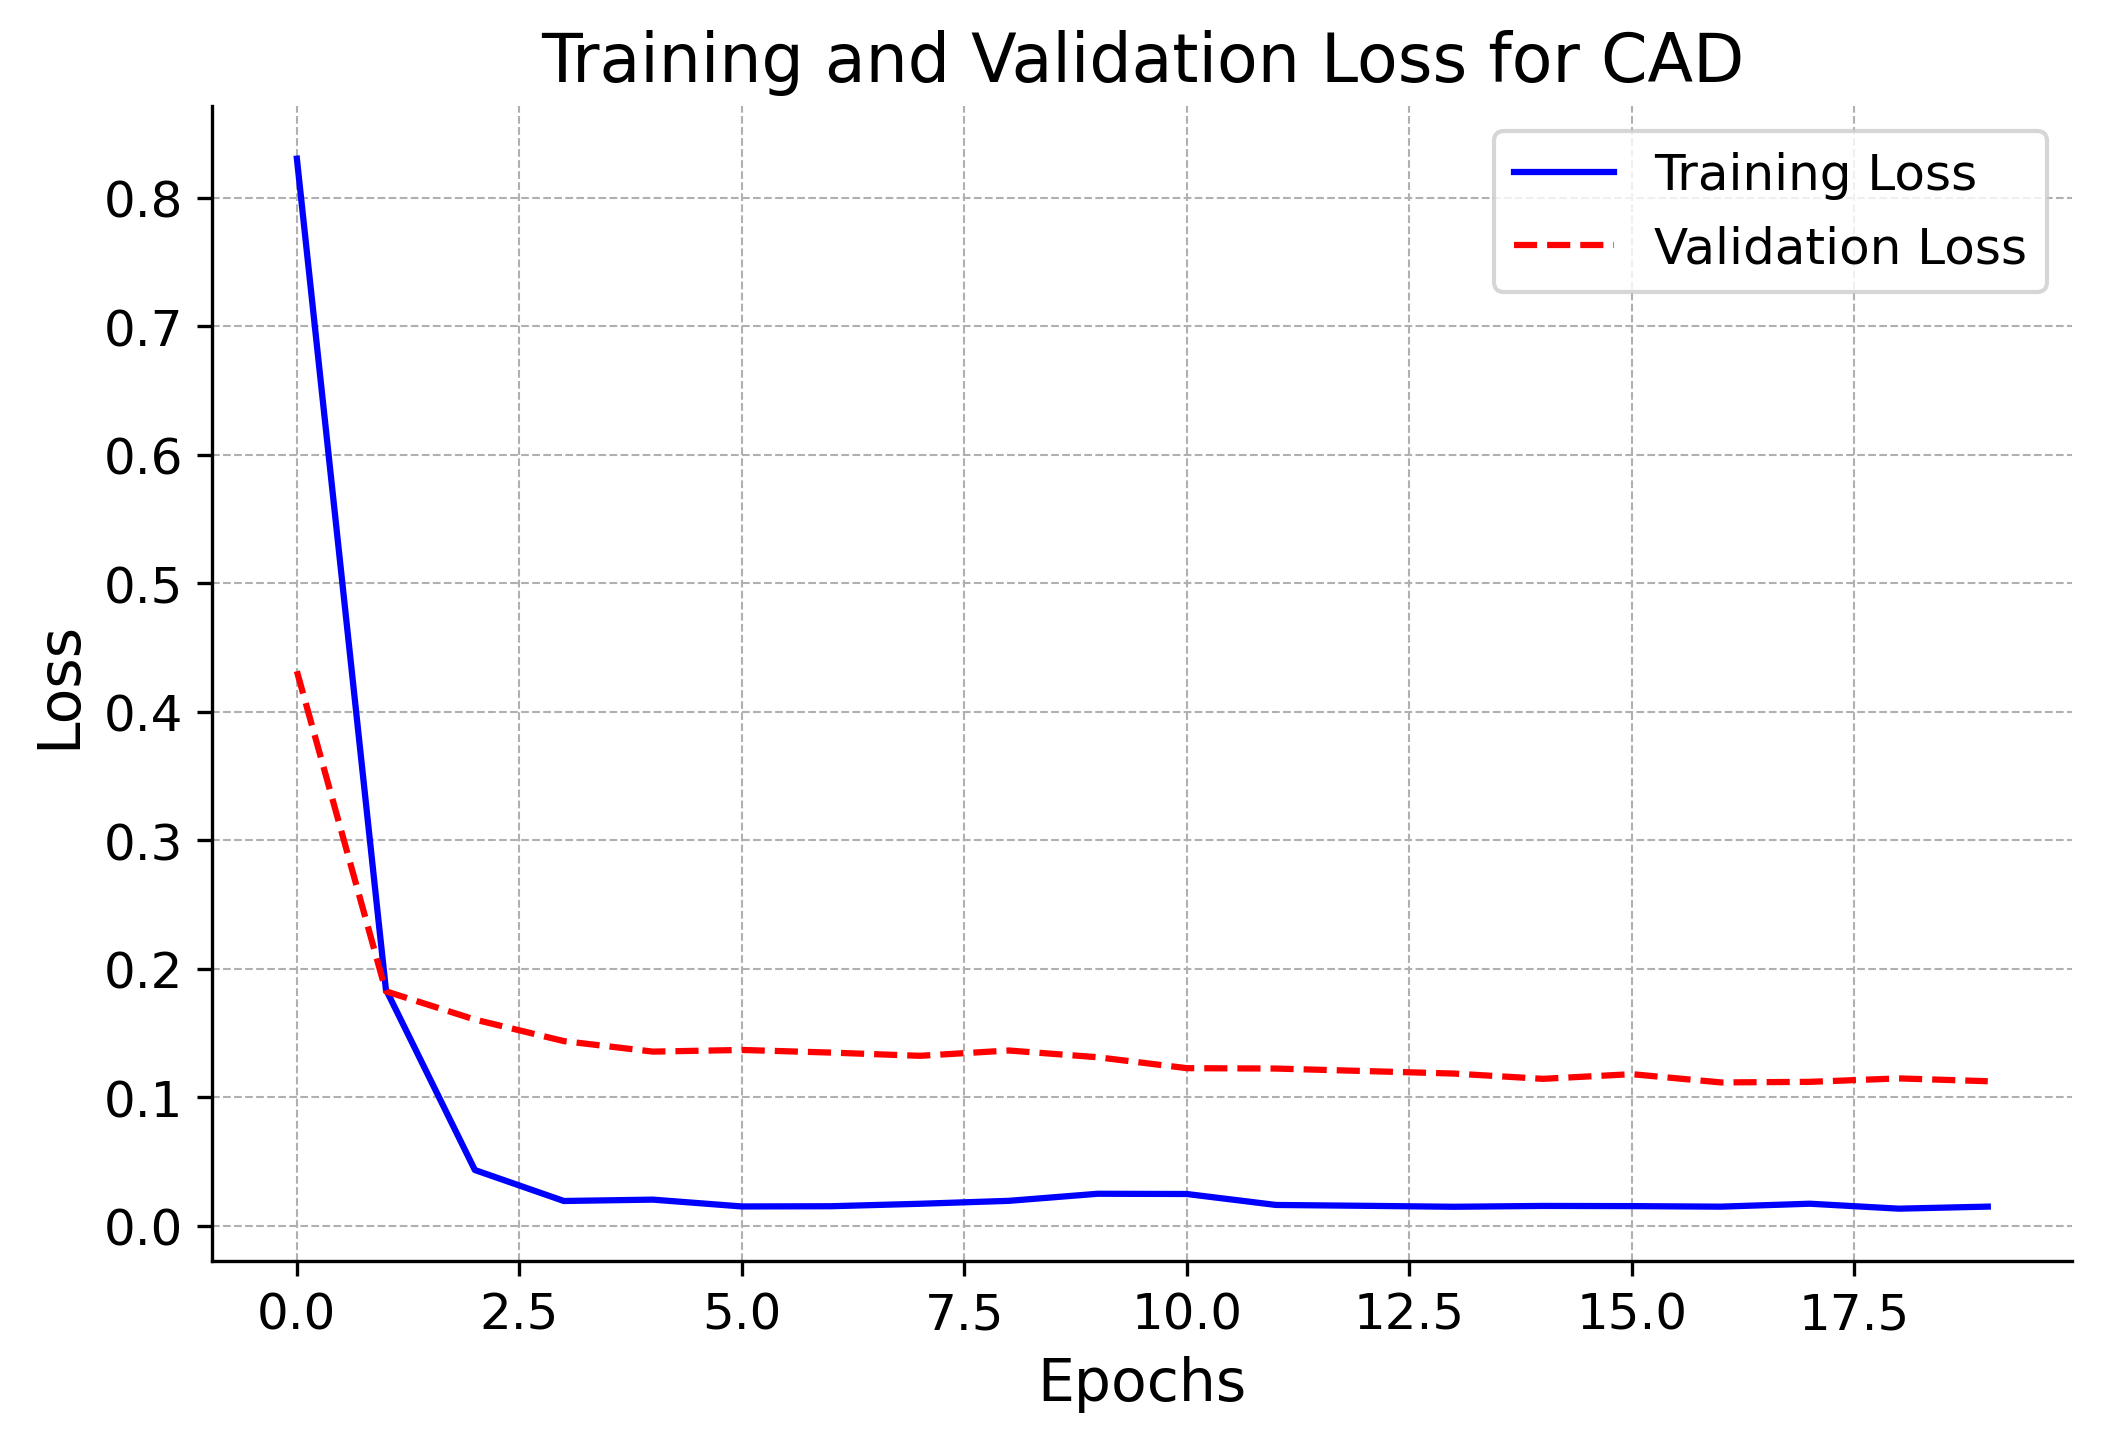
\includegraphics[width=\linewidth]{plots/CAD_loss_plot.png}
    \end{column}
    \begin{column}{0.25\textwidth}
        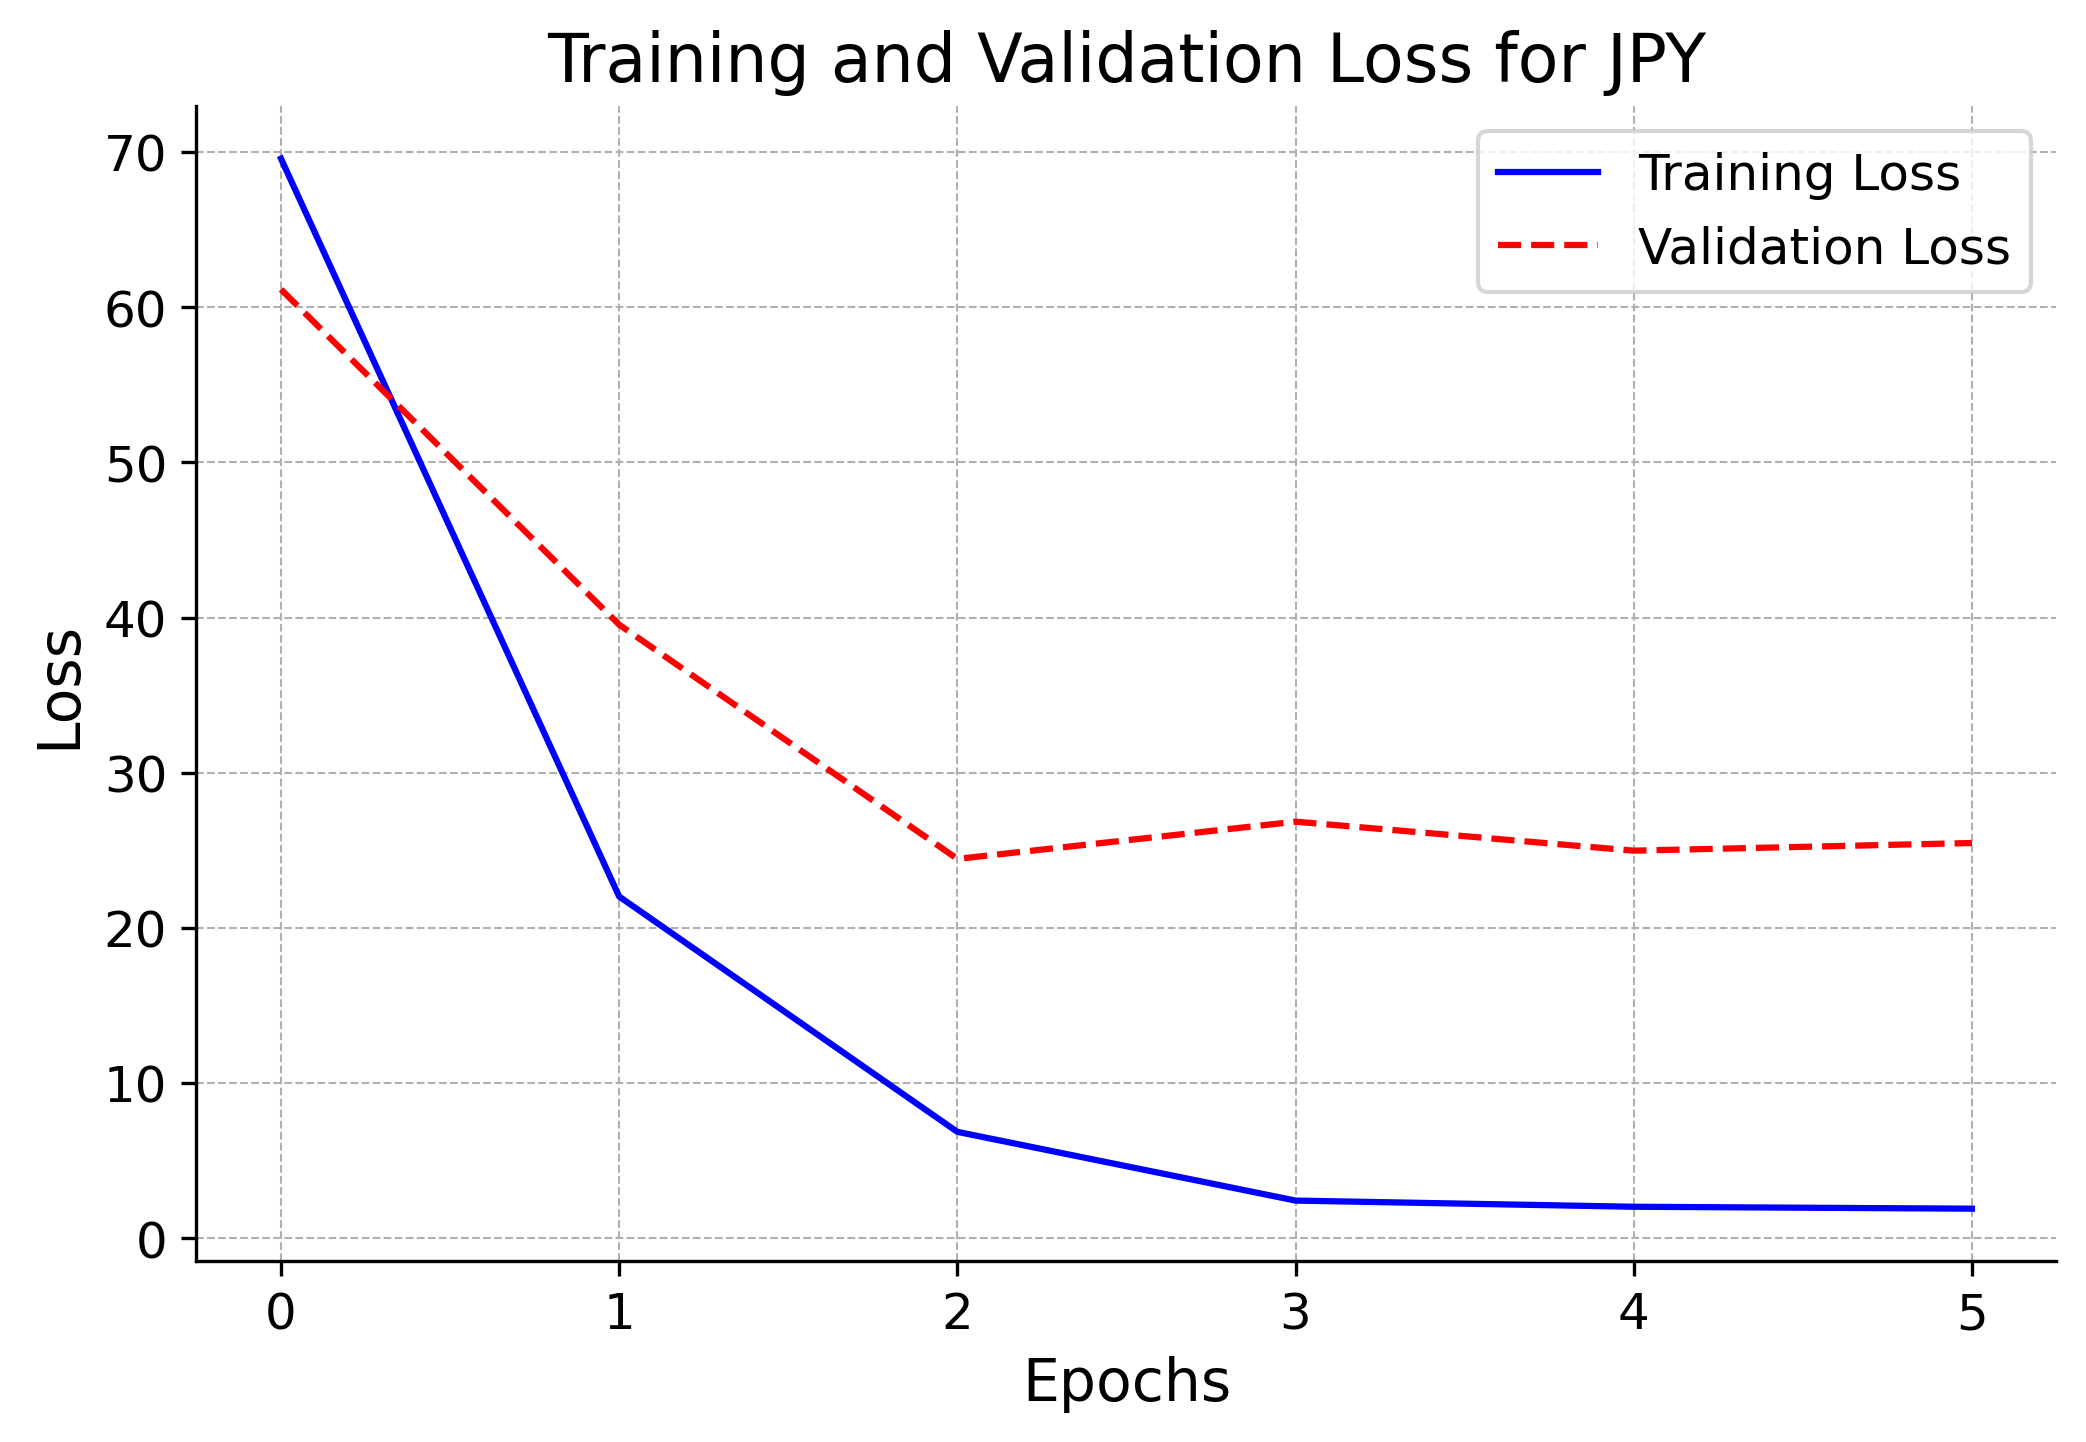
\includegraphics[width=\linewidth]{plots/JPY_loss_plot.png}
    \end{column}
    \begin{column}{0.25\textwidth}
        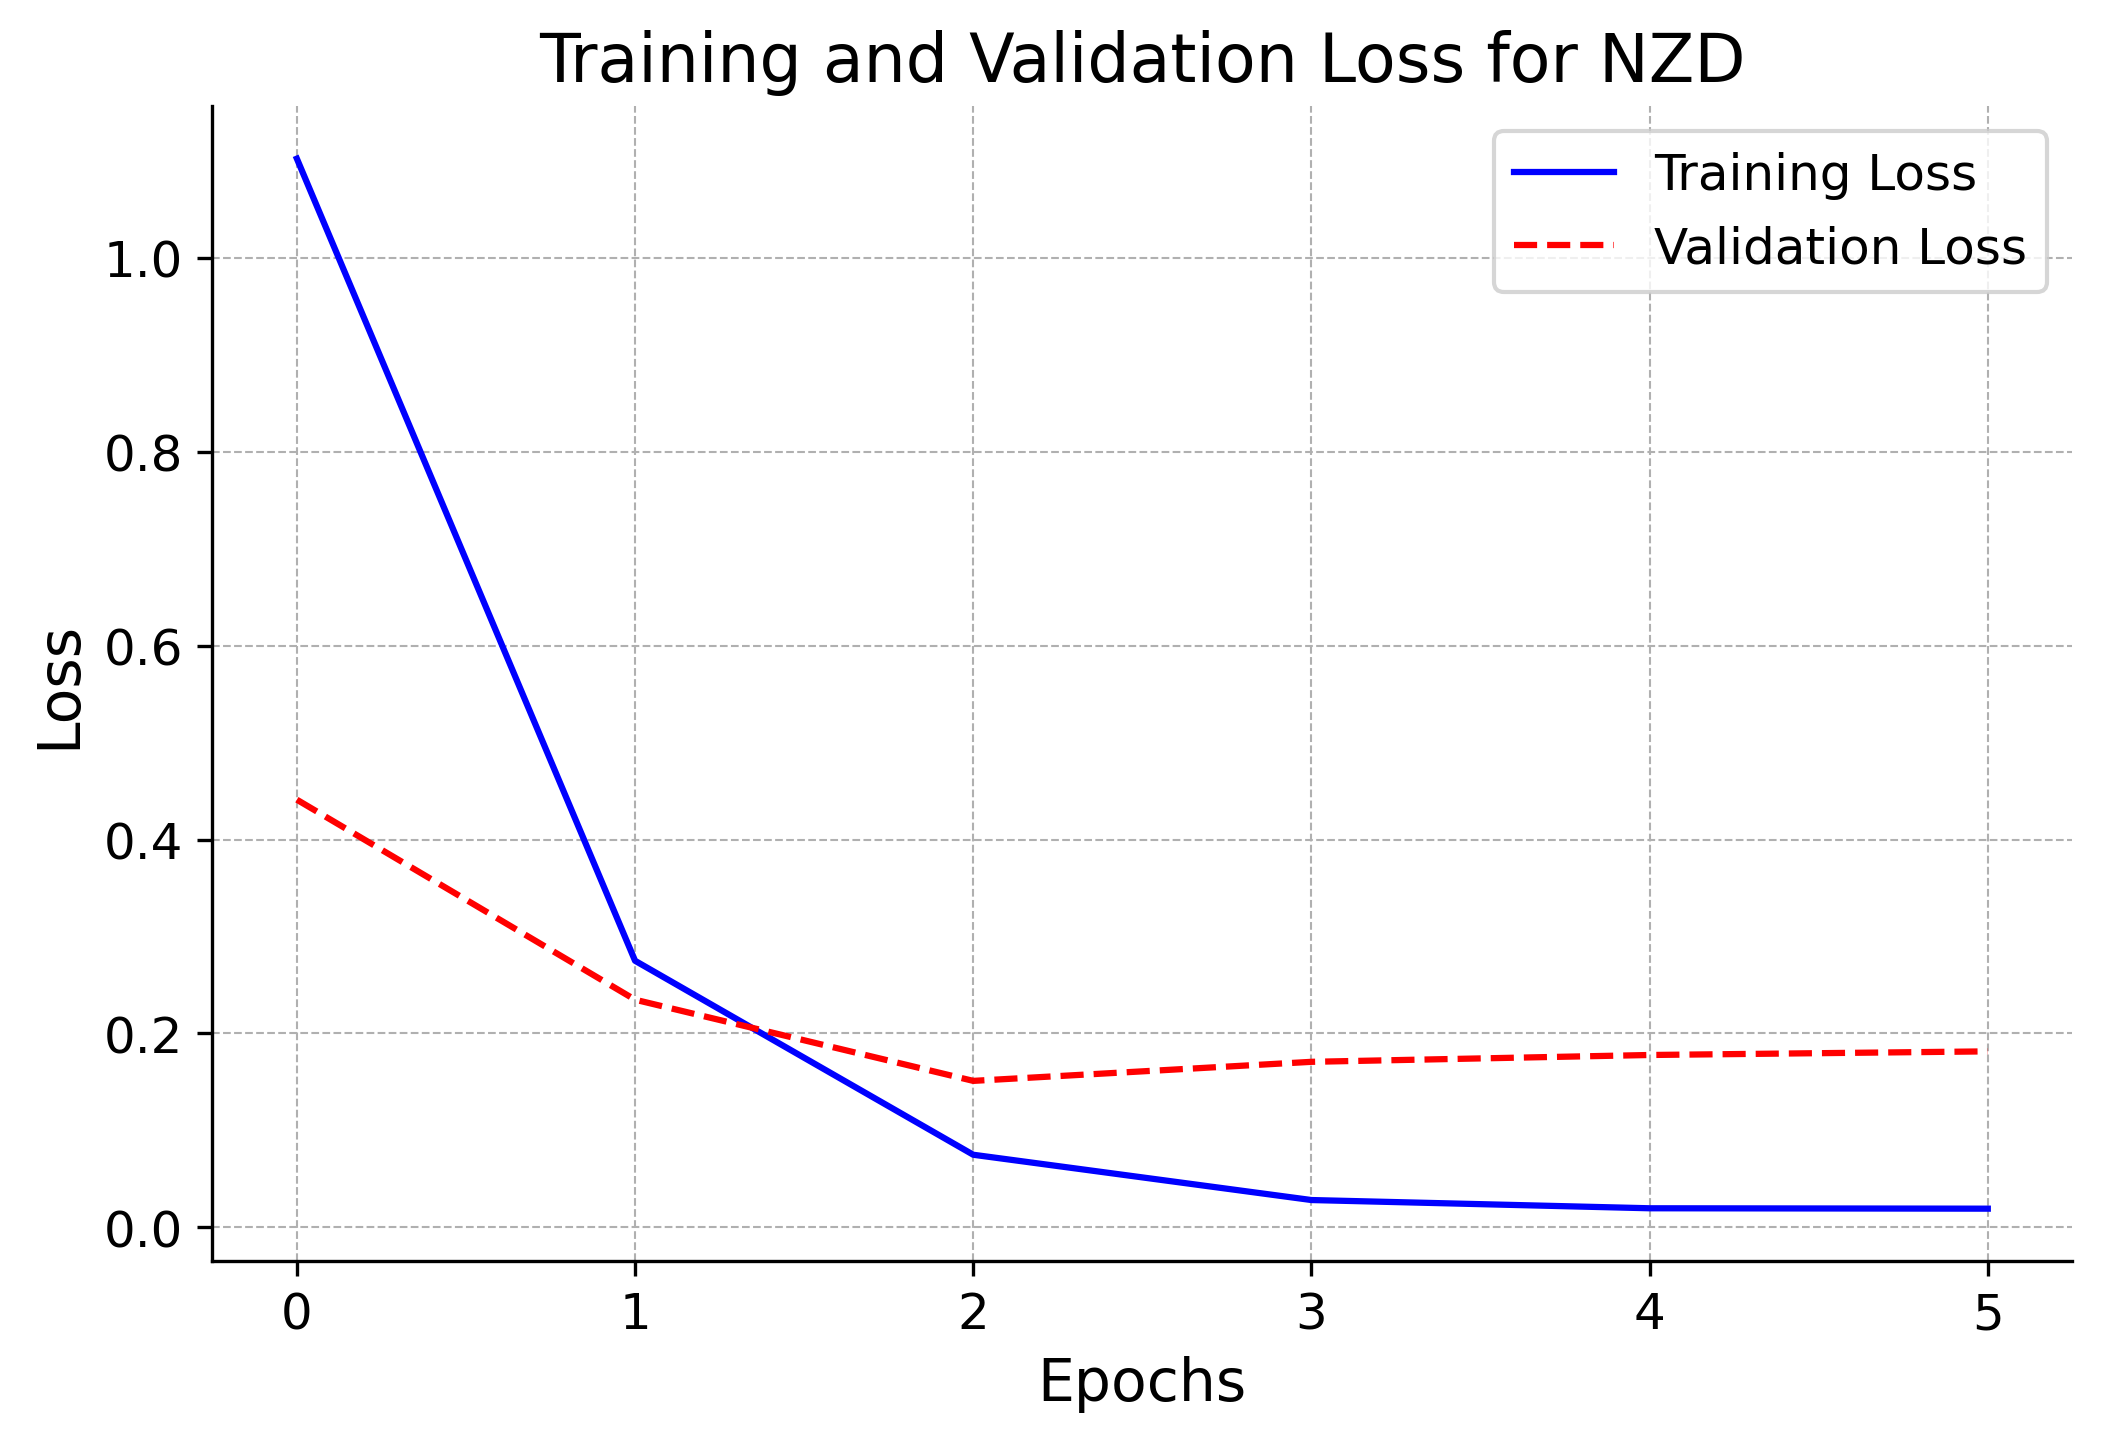
\includegraphics[width=\linewidth]{plots/NZD_loss_plot.png}
    \end{column}
    \begin{column}{0.25\textwidth}
        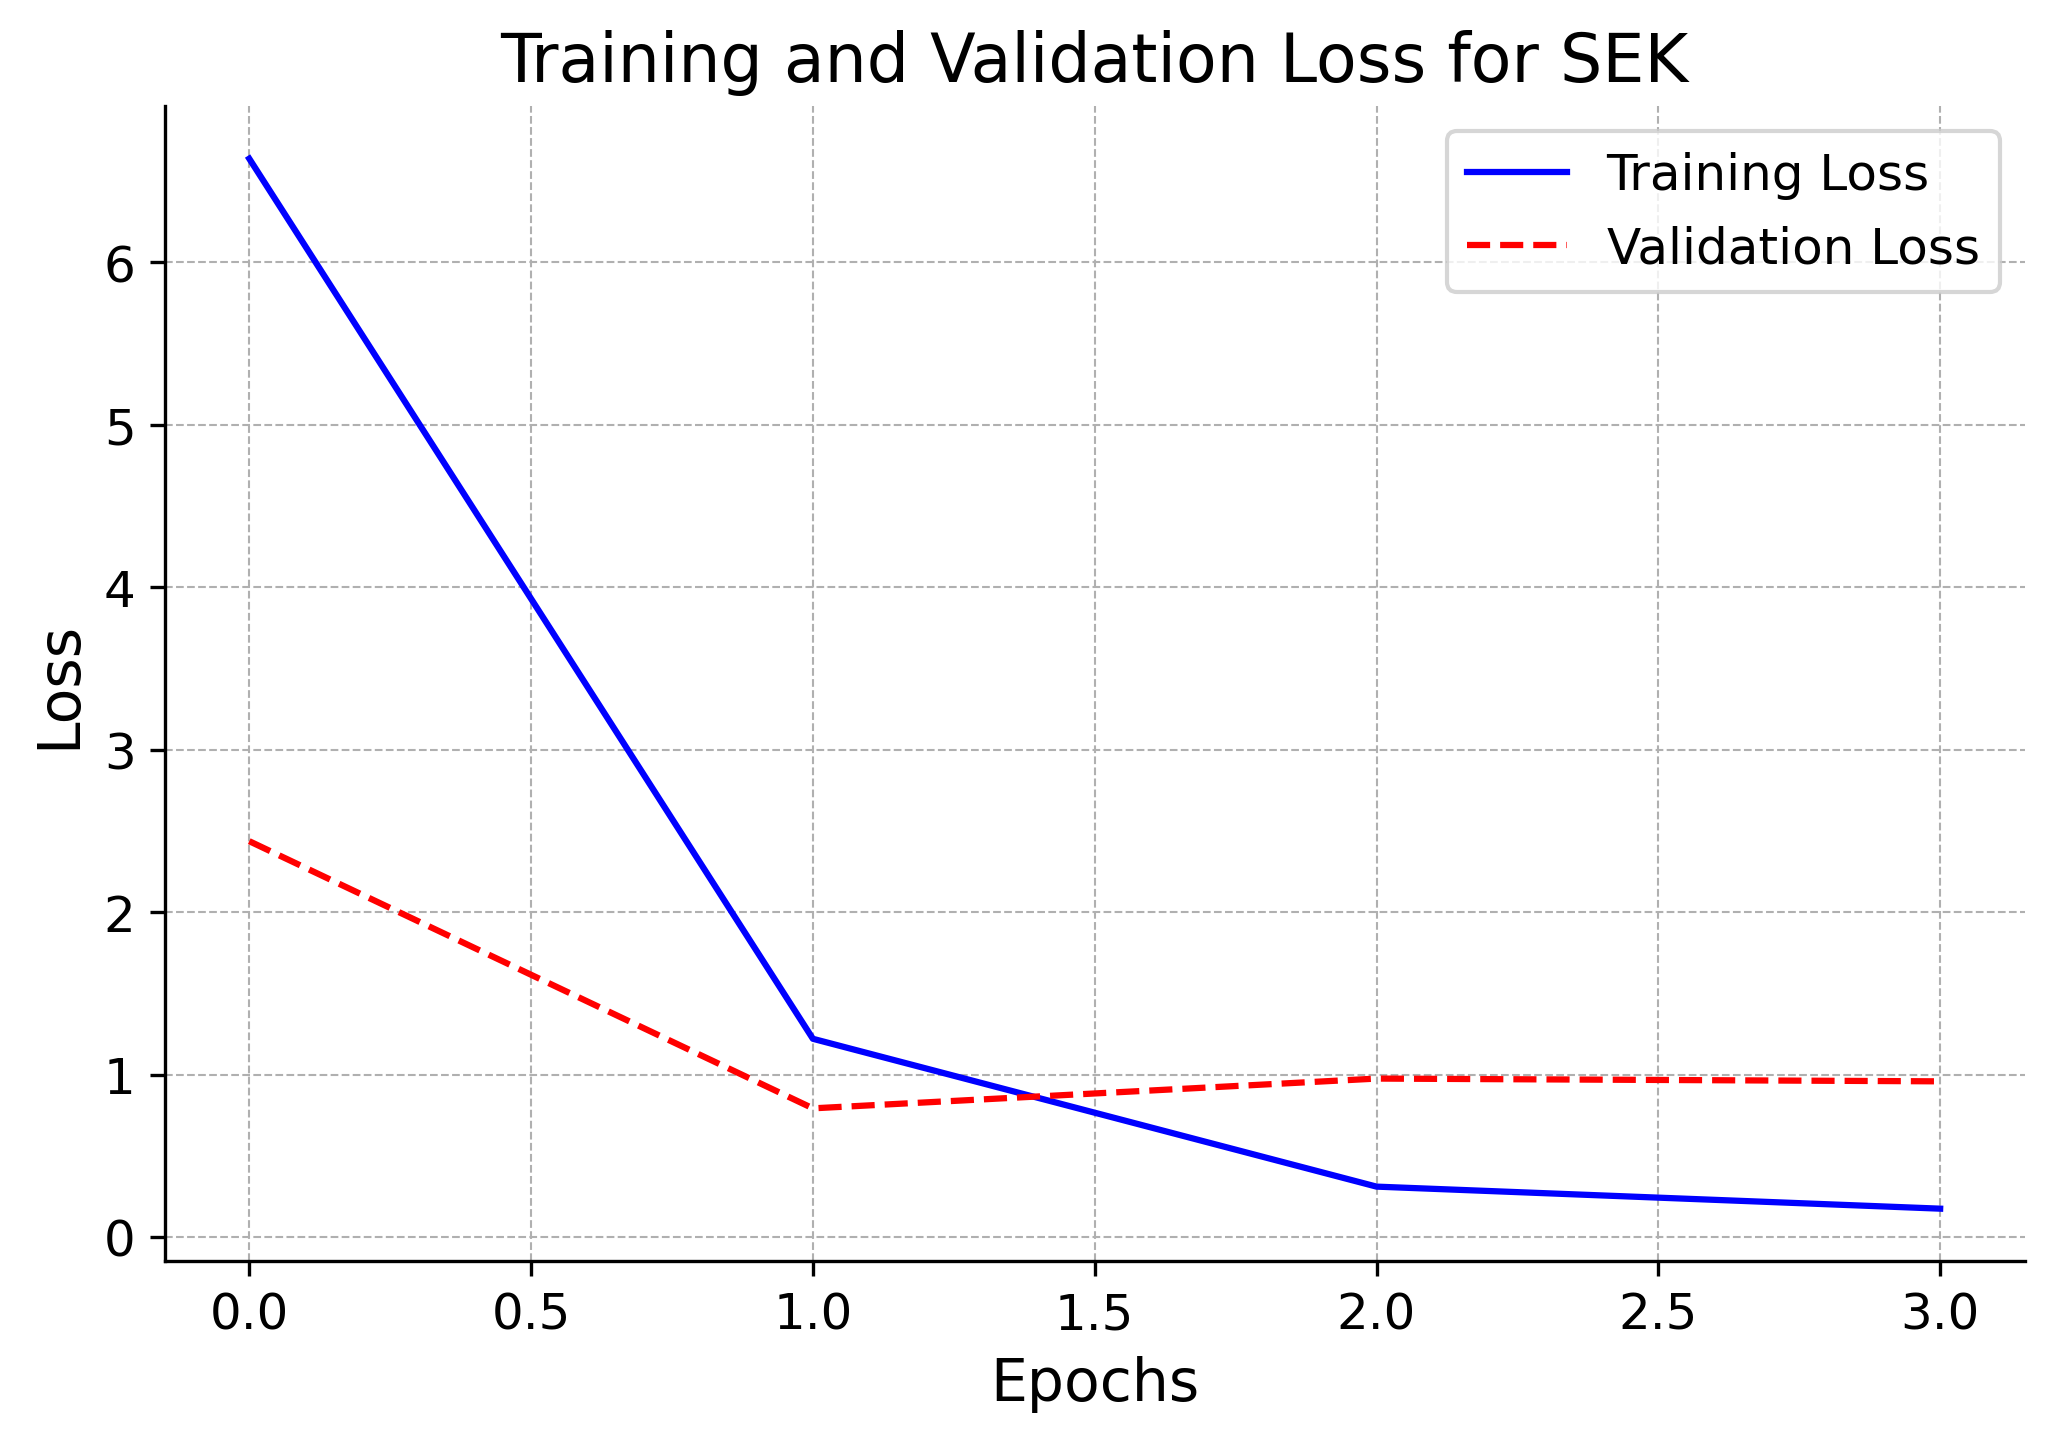
\includegraphics[width=\linewidth]{plots/SEK_loss_plot.png}
    \end{column}
\end{columns}
\end{frame}

\section{Comparison with Benchmark}

\begin{frame}{Average performance estimators}
\begin{table}\centering
\ra{1.3}
\caption{Averaged performance estimators for daily and weekly frequencies}\label{tab:res}
\begin{tabular}{@{}rrrcrr@{}}\toprule
& \multicolumn{2}{c}{Daily} & \phantom{abc}& \multicolumn{2}{c}{Weekly}\\
\cmidrule{2-3} \cmidrule{4-6}
& \textit{sMAPE(\%)} & \textit{MSE} && \textit{sMAPE(\%)} & \textit{MSE} \\
\midrule
S-CNN & 59.70  & 0.006 && 81.45 & 0.010 \\
ES-RNN & 13.72 & 560.580 && 7.96 & 323.021\\
V-AR & 0.83 & 0.001 && 2.24 & 0.000\\
\bottomrule
\end{tabular}
\end{table}
\end{frame}

\section{Conclusions}

\begin{frame}[allowframebreaks]{Conclusion and Key Findings}
        \begin{itemize}
            \item Explored the synergy between neural networks and traditional statistical models for forex forecasting.
            \item ES-RNN and S-CNN were both outperformed by Vector Autoregression (V-AR).
            \item Identified a positive bias issue in the ES-RNN due to an ineffective training loss function.
            \item S-CNN struggled with non-stationary and insufficient data.
            \item Emphasised the importance of ample data and the effectiveness of simpler, classic statistical methods.
        \end{itemize}
    \newpage
    \begin{center}
        \textsc{\textbf{Future Steps}}
    \end{center}
        \begin{itemize}
            \item Explore alternative loss function, and input window, for ES-RNN to mitigate bias in predictions.
            \item Train the ES-RNN with all the series to exploit shared parameters and learn common local trends among the series.
            \item Address data non-stationarity and volume issues to enhance the performance of complex models.
        \end{itemize}
\end{frame}

\begin{frame}[allowframebreaks]{References}

  \bibliography{demo}
  \bibliographystyle{abbrv}

\end{frame}

\end{document}
